\section{Methods}
\label{sec:methods}

Five horses were equipped with nine ProMove-mini IMUs (Inertia Technology B.V., Enschede, The Netherlands) on the sacrum, withers, poll, each limb, and both tuber coxae. The measurement range of the low-g accelerometer was $\pm16 g$, while the gyroscope could measure angular velocity within the range of $\pm2000$ degrees per second. The \gls{imu}s on both tuber coxae were attached directly to the skin using double-sided adhesive tape. The limbs \gls{imu}s were fitted inside custom pockets, and the pockets were wrapped firmly around the boots (on cannon bone) using Velcro straps, positioning the \gls{imu}s on the distal aspect of limbs. The poll \gls{imu} was mounted on a customized cap, while the withers \gls{imu} was placed on a girth. 

One of the primary objectives of this study was to compare the outcome of pelvis roll angle calculation obtained from sacrum \gls{imu} and \gls{omc}. To achieve this comparison, it was essential to translate the orientation of the sacrum \gls{imu} in three dimensions and this translation required at least three markers for accurate assessment \cite{Strang2016Calculus3}. In geometrical terms, we conceptualized the sacrum \gls{imu} as a plane and the markers as points. However, a significant challenge arose due to the limited surface area of the small \gls{imu}. Even if it were possible to fit three markers, they would be closely grouped together, causing the cameras to detect them as a single, large marker. 

To address the \gls{imu} small surface and the limited capability of the cameras, a specifically designed rigid plate, following the natural curve shape of the horse's pelvis, was securely attached to the sacrum using adhesive tapes, as depicted in the bottom right section of Figure \ref{bigpic}). This rigid plate effectively enlarged the available surface for marker placement, making it feasible to attach three markers onto the rigid plate instead of the \gls{imu}. These three rigid body markers were henceforth referred to as the 'rigid triad of markers.' Positioned on top of the rigid body and centrally aligned with the sacrum, the sacrum \gls{imu} was placed. The x and z-axes of the sacrum \gls{imu} were aligned horizontally (in the direction of the horse's forward movement) and vertically (perpendicular to the sacrum). The precise positions of the \gls{imu}s are illustrated in Figure \ref{bigpic}.

On the top and in the center of withers, poll, sacrum, and both tuber coxae \gls{imu}s, spherical reflective markers (25 mm diameter) were attached using double-sided adhesive tape. The center marker (on top of the actual sacrum \gls{imu}) was not used for this study.


\begin{figure}[tb]

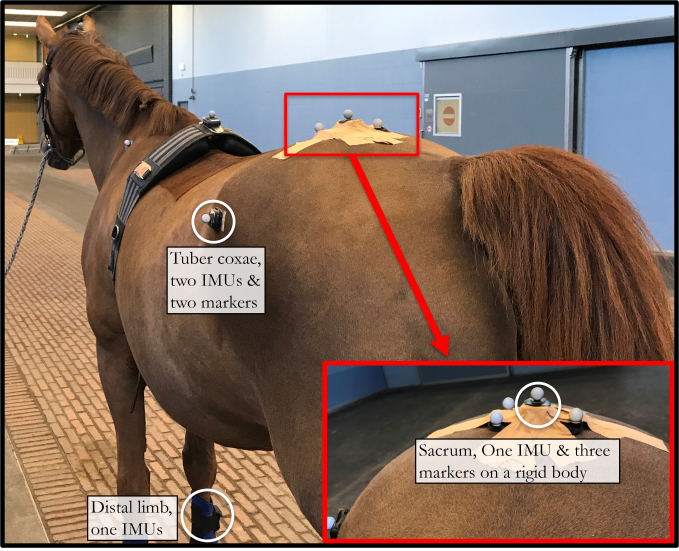
\includegraphics[width=.95\linewidth]{chapters/Pelvis/figures/1.jpg}
\caption{Constellation of the sacrum and left tuber coxae markers and \gls{imu}s, and the rigid triad of markers (right bottom). The center marker on the rigid triad of markers was not used in this study}
\label{bigpic}
\end{figure}

 
%\begin{figure}[htbp]
%\centering
%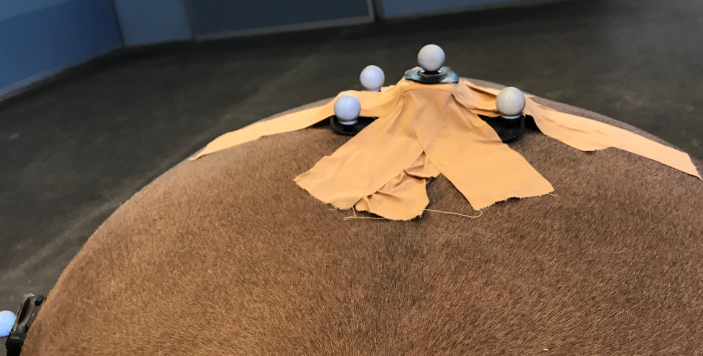
\includegraphics[width=.95\linewidth]{chapters/Pelvis/figures/IMG_4390.png}
%\caption{Rigid triad of markers on sacrum. The center marker was not used in this study}
%\label{smallpic}
%\end{figure}

Each horse was walked and trotted in hand along a straight line on a hard surface. \gls{omc} data were recorded using Qualisys \gls{omc} software, connected to twenty eight cameras. The data collection frequency of \gls{imu} and \gls{omc} were the same at 200 Hz. After the data collection, \gls{imu} and \gls{omc} outputs were time-synchronized. In addition, The signals derived from the \gls{imu} were low-pass filtered (fourth-order Butterworth filter and 30 Hz cut-off frequency) to reduce any potential noise artifacts and enhance the quality of the signals  \cite{456}. 

Our goal was to compare the methods and measurement devices within one stride. Therefore, \gls{imu} and \gls{omc} data were split into strides using the technique in chapter \ref{chapter:Step}. This stride segmentation allowed us to focus our analysis on the specific events and intricacies occurring within each stride. Then, in order to make these data streams directly comparable, all collected strides were uniformly time-scaled to consist of precisely 100 timesteps each. Subsequently, the vertical displacements of both tuber coxae \gls{imu}s were calculated using a previously validated algorithm from a study \cite{pfau_2005_a}. Finally, the pelvis roll angle was calculated for each stride using two methods and two measuring devices, which summed up to four separate calculations: 

\vspace{0.4cm}

\textbf{Roll method:} Rotation angle (Raw Euler angle signal around x-axis extracted directly from sacrum \gls{imu}, or rotation angle of the rigid plate (around x-axis of sacrum \gls{imu}) using the displacements of the rigid triad of markers.

The orientation of a rigid body in space can be determined uniquely from the positions of at least three points on the body since the orientation of the body is completely specified by the relative positions of these three points. One common method for determining the orientation of a rigid body from three points is to use the cross-product. The cross product of two vectors is a vector that is perpendicular to both of the original vectors. This means that the cross-product of any two vectors from the three points will lie along the axis of rotation of the body. Once the axis of rotation has been determined, the angle of rotation can be found using the dot product. The dot product of two vectors is a scalar that measures the amount of overlap between the two vectors. In this case, the dot product of the axis of the rotation vector and one of the original vectors will give the angle of rotation between the two vectors.

\vspace{0.4cm}

\textbf{Inverse sine method:} The angle between the horizontal plane of the horses and the line crosses both tuber coxae \gls{imu}s or both tuber coxae markers, as presented in Figure \ref{pfau}: 

\begin{equation}
    a = arcsin([Z_{RTC} + Z_{LTC}]/d)
\end{equation}

\begin{figure}[htbp]
\centering
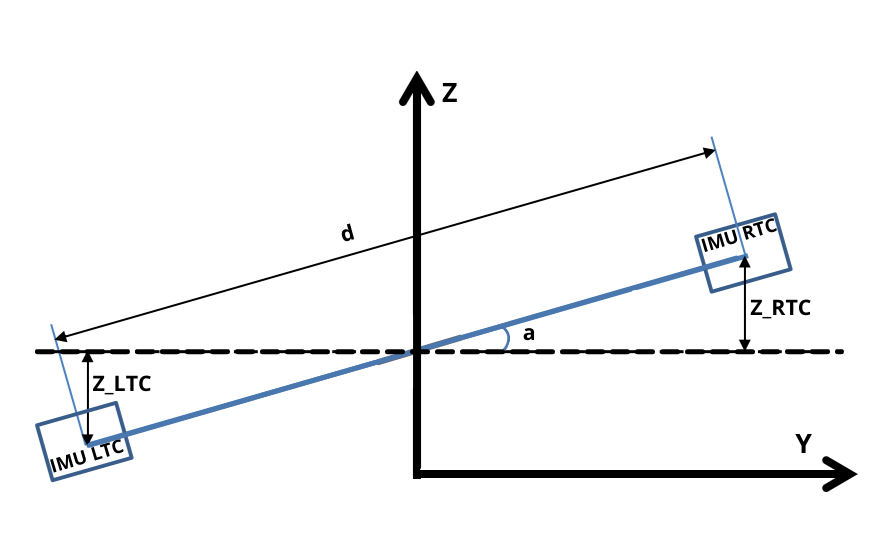
\includegraphics[width=.75\linewidth]{chapters/Pelvis/figures/Z_RTC (1).png}
\caption{Calculation of pelvis roll angle (a) using vertical displacement of right and left tuber coxae (RTC and LTC) and the three-dimensional distance between tuber coxae (d)}
\label{pfau}
\end{figure}

For method validation and comparison, \gls{rmse} of pelvis roll angle (in degree) was calculated between methods and measurement devices as follows,

\begin{equation}
RMSE = \sqrt{\frac{1}{n} \sum_{i=1}^{n} (Angle_{Stride_i,IMU} - Angle_{Stride_i,OMC})^2}
\end{equation}

Finally, a Bland-Altman analysis was performed within the methods and between the measurement devices, and also between the methods using each measurement device \cite{456}. The limits of agreement between methods were reported in degrees as 

\begin{equation}
[\text{bias}, 2\times \text{standard deviation}]
\end{equation}

